\documentclass[letterpaper,
               keeplastbox,
               %boxit,
               %titlepage,   % separate title page
               %refpage      % separate references
               nospread,
               biblatex,
              ]{jacow}
%
% CHANGE SEQUENCE OF GRAPHICS EXTENSION TO BE EMBEDDED
% ----------------------------------------------------
% test for XeTeX where the sequence is by default eps-> pdf, jpg, png, pdf, ...
%    and the JACoW template provides JACpic2v3.eps and JACpic2v3.jpg which
%    might generates errors, therefore PNG and JPG first
%
\makeatletter%
	\ifboolexpr{bool{xetex}}
	 {\renewcommand{\Gin@extensions}{.pdf,%
	                    .png,.jpg,.bmp,.pict,.tif,.psd,.mac,.sga,.tga,.gif,%
	                    .eps,.ps,%
	                    }}{}
\makeatother

% CHECK FOR XeTeX/LuaTeX BEFORE DEFINING AN INPUT ENCODING
% --------------------------------------------------------
%   utf8  is default for XeTeX/LuaTeX 
%   utf8  in LaTeX only realises a small portion of codes
%
\ifboolexpr{bool{xetex} or bool{luatex}} % test for XeTeX/LuaTeX
 {}                                      % input encoding is utf8 by default
 {\usepackage[utf8]{inputenc}}           % switch to utf8

\usepackage[USenglish]{babel}

\usepackage[final]{pdfpages}
\usepackage{multirow}
\usepackage{ragged2e}

% Packages to comment out before final release:
\usepackage{todonotes}
\presetkeys{todonotes}{inline}{}
% END packages to comment out before final release
\usepackage{subcaption}
%
% if BibLaTeX is used
%
\ifboolexpr{bool{jacowbiblatex}}%
 {%
  \addbibresource{napac2022.bib}
 }{}
\listfiles


%
% command for typesetting a \section like word
%
\newcommand\SEC[1]{\textbf{\uppercase{#1}}}

%%
%%   Lengths for the spaces in the title
%%   \setlength\titleblockstartskip{..}  %before title, default 3pt
%%   \setlength\titleblockmiddleskip{..} %between title + author, default 1em
%%   \setlength\titleblockendskip{..}    %afterauthor, default 1em

%\copyrightspace %default 1cm. arbitrary size with e.g. \copyrightspace[2cm]

% testing to fill the copyright space
%\usepackage{eso-pic}
%\AddToShipoutPictureFG*{\AtTextLowerLeft{\textcolor{red}{COPYRIGHTSPACE}}}

\begin{document}

\title{Measurements of the five-dimensional phase space distribution of an intense ion beam}

\author{A. Hoover\thanks{hooveram@ornl.gov}, K. Ruisard, A. Alexandrov, A. Zhukov, S. Cousineau, ORNL, Oak Ridge, Tennessee, USA}
	
\maketitle

%
\begin{abstract}
No simulation of intense beam transport has accurately reproduced measurements at the level of beam halo. One potential explanation of this discrepancy is a lack of knowledge of the initial distribution of particles in six-dimensional (6D) phase space. A direct 6D measurement of an ion beam was recently performed at the Spallation Neutron Source (SNS) Beam Test Facility (BTF), revealing nonlinear transverse-longitudinal correlations in the beam core that affect downstream evolution. Unfortunately, direct 6D measurements are limited in resolution and dynamic range; here, we discuss the use of three slits and one screen to measure a 5D projection of the 6D phase space distribution, overcoming these limitations at the cost of one dimension. We examine the measured 5D distribution before and after transport through the BTF and compare to particle-in-cell simulations. We also discuss the possibility of reconstructing the 6D distribution from 5D and 4D projections.
\end{abstract}

\section{Introduction}


The performance of high-intensity particle accelerators is limited by beam halo formation \cite{}. Attempts to reproduce measured beam distributions at the halo level — a density at or below 10$^{-4}$ relative to the beam core — have been unsuccessful \cite{LEDA, Groening}. This is likely due to an inaccurate initial distribution of particles in 6D phase space. 

The Spallation Neutron Source (SNS) Beam Test Facility (BTF) is poised to resolve these discrepancies. The BTF is a replica of the front-end of the SNS linac — the H$^-$ ion source, low-energy beam transport (LEBT), radio-frequency quadrupole (RFQ), and medium energy beam transport (MEBT) — followed by a twenty-cell FODO transport line \cite{}. There are two emittance measurement stations: one after the RFQ and one after the FODO line. The two-dimensional (2D) horizontal and vertical phase space distributions can be measured at either station with a dynamic range above $10^6$ \cite{Alexandrov2020}, large enough to image the beam halo. The 6D phase space distribution can be measured at the first station. 

The goal of the BTF experimental program is to reproduce the measured halo at the second emittance station in simulation. To do so will require an accurate model of the accelerator and a realistic initial bunch. Unfortunately, it is not currently possible to generate a realistic initial bunch due to the limited dynamic range ($10^1$) and resolution (10 points per dimension) of the 6D measurement \cite{CatheyPRL}. Improvements to the scan efficiency are under development. In this paper, we discuss the use of three slits and one screen to measure a 5D projection of the 6D phase space distribution, overcoming these limitations at the cost of one dimension. 

\section{Efficient 5D phase space measurement}

The measurement apparatus consists of two vertical slits to select the horizontal position $x$ and momentum $x'$, a vertical slit to select the vertical position $y$, and a scintillating screen after a dipole bend (see \cite{Ruisard2022-NAPAC}). The vertical momentum $y'$ is linearly related to the vertical position on the screen; the energy deviation $w$ is a function of the horizontal position on the screen and the $x$ and $x'$ selected by the upstream slits. The scan consists of a series of "sweeps" where the vertical slits are held fixed while the horizontal slit moves at a fixed speed, collecting the image on the screen on every beam pulse. A rectilinear scan pattern is employed with a linear correlation between $x$ and $x'$ to align the grid with the $x$-$x'$ distribution. The data is linearly interpolated onto a regular grid after transforming to phase space variables.

% \begin{figure}[!t]
%     \centering
%     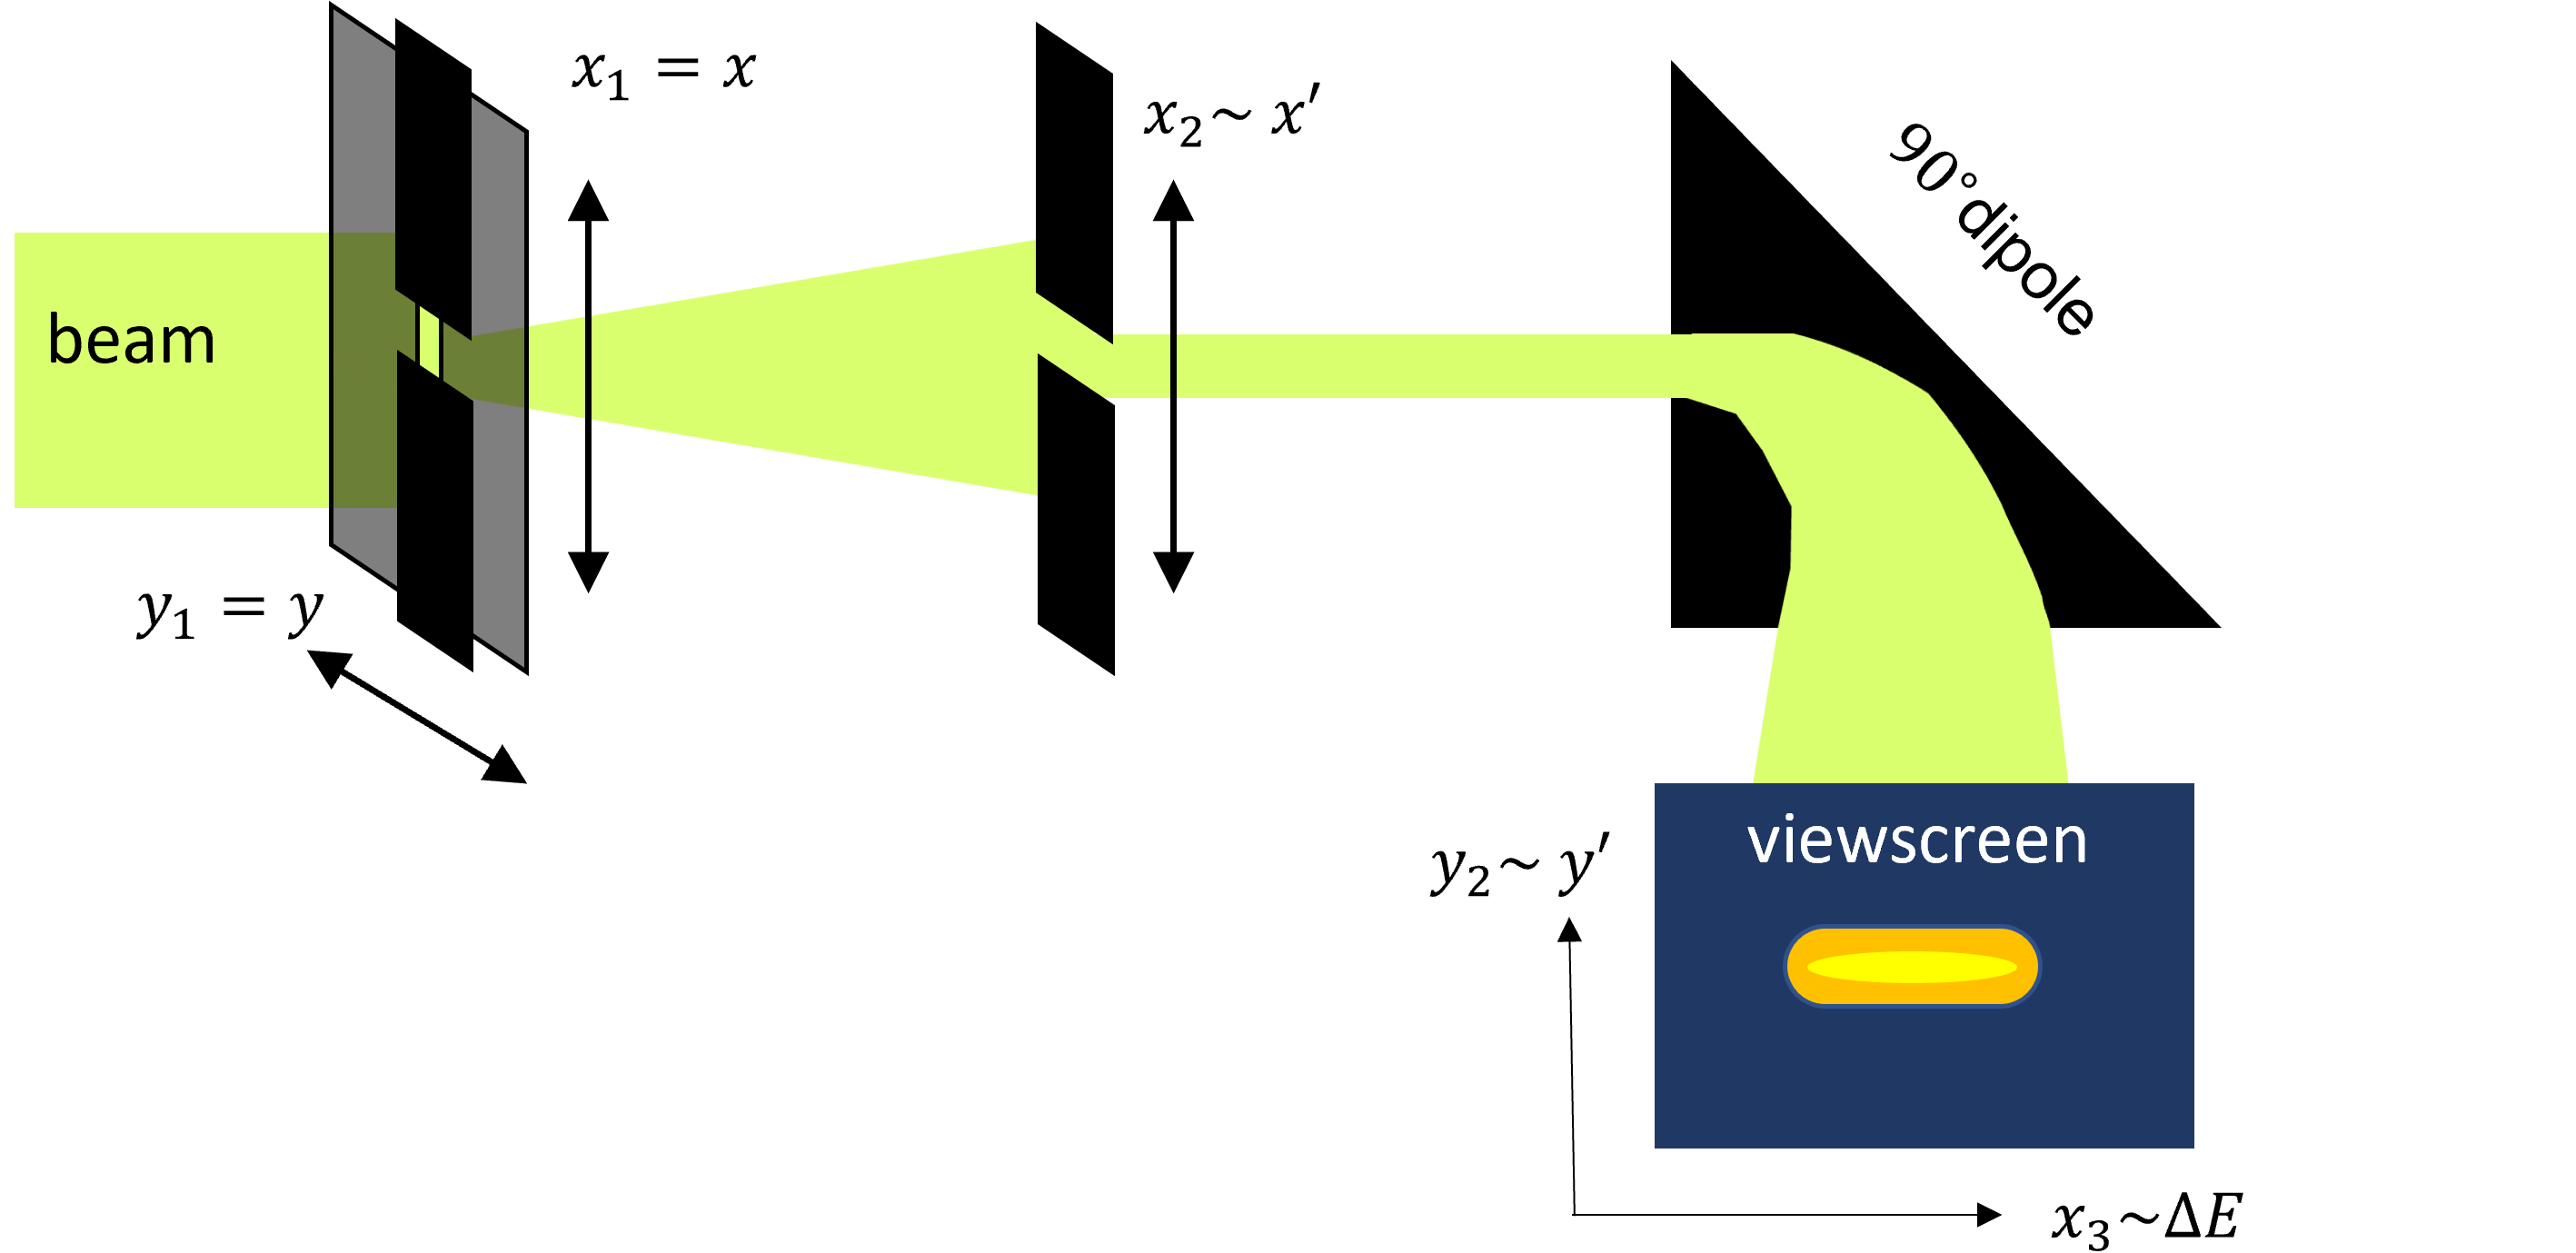
\includegraphics[width=\columnwidth]{apparatus5D.png}
%     \caption{5D phase space measurement apparatus.}
%     \label{fig:5dmeas}
% \end{figure}



\section{Measurements of the initial distribution in the BTF}

\subsection{Revisiting hidden features in the beam core}

We first examine the measured 5D distribution at the first emittance station. The beam current during the measurement was stable at [] mA. [] points were collected over [] hours as the slits traversed a ? x ? x ? grid. Fig.~\ref{fig:VS06_corner} shows the 2D projections of the measured 5D phase space distribution. The density profiles vary smoothly in all projections and there are apparently no inter-plane correlations.
%
\begin{figure}[!b]
    \centering
    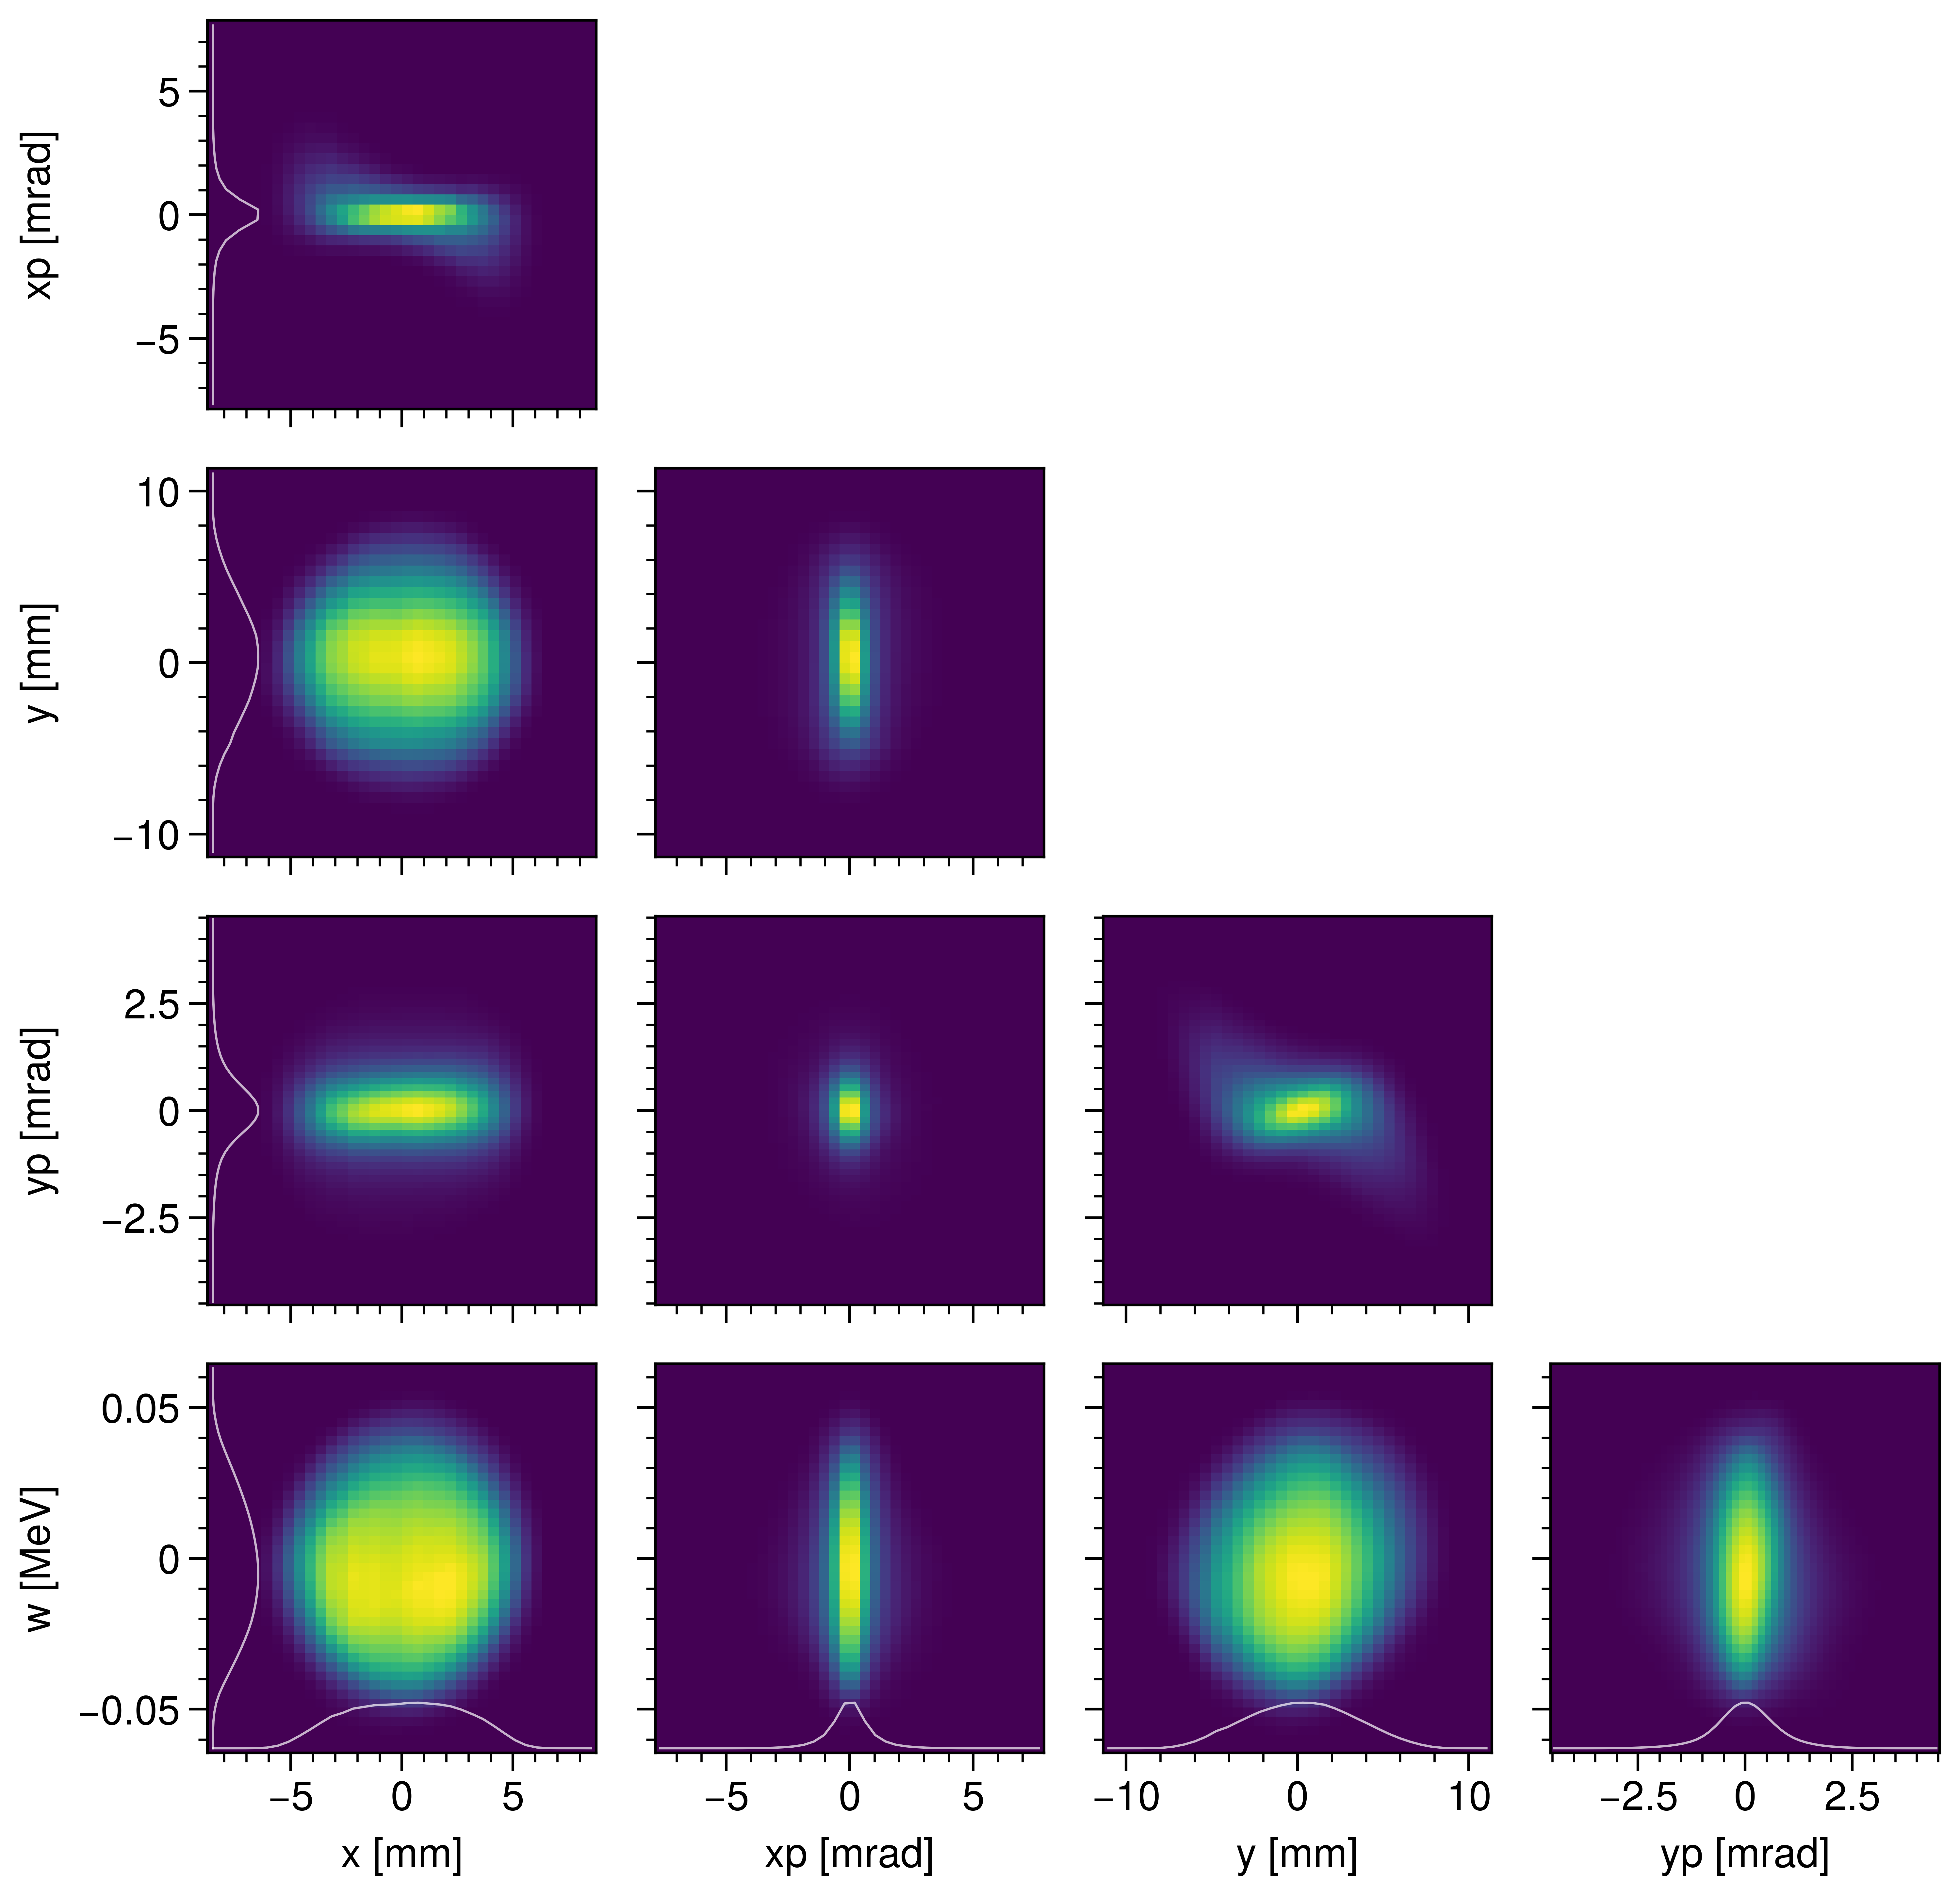
\includegraphics[width=\columnwidth]{VS06_corner.png}
    \caption{1D and 2D projections of the measured 5D phase space distribution at the first emittance station in the BTF.}
    \label{fig:VS06_corner}
\end{figure}
%

Previous bunch shape monitor (BSM) measurements of the beam exiting the RFQ have revealed nonlinear transverse-longitudinal correlations in the beam core: the energy distribution of particles at the center of transverse phase space ($x \approx x' \approx y \approx y' \approx 0$) is hollow and bimodal while the full projection is unimodal \cite{CatheyPRL}. This is a space-charge-driven effect \cite{Ruisard2021-hollow} and has a clear dependence on the beam intensity (see Appendix \ref{app:A}). These studies examined the relationship between the energy and transverse coordinates by slicing the distribution in the transverse plane before projecting the distribution onto the energy axis; i.e., by inserting one or more slits upstream of the BSM. The five-dimensional nature of the correlation is made clear by observing the energy profile as each dimension is sliced. We repeat this for our 5D measurement in Fig.~\ref{fig:hollow_a}.
%
\begin{figure}[!t]
    \centering
    \begin{subfigure}{\columnwidth}
        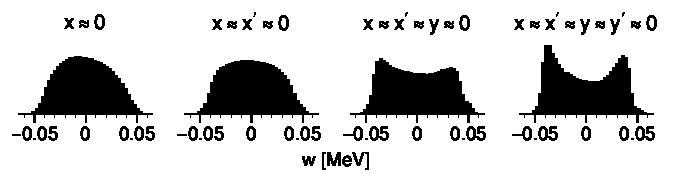
\includegraphics[width=\textwidth]{w_slices.pdf}
        \caption{}
        \label{fig:hollow_a}
    \end{subfigure}
    \begin{subfigure}{\columnwidth}
        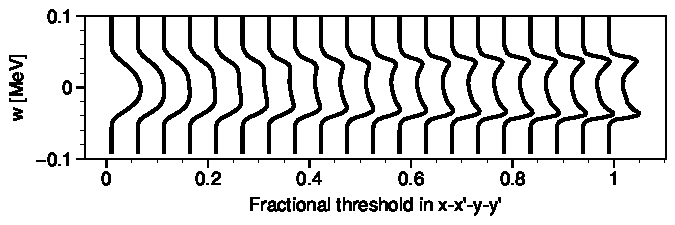
\includegraphics[width=\textwidth]{4Dcontour_dE2.pdf}
        \caption{}
        \label{fig:hollow_b}
    \end{subfigure}
    \caption{Hollow energy distribution in the beam core measured at the first emittance station in the BTF. (a) Energy projection of the 5D phase space distribution as it is sliced in transverse phase space. (b) Each curve is the energy distribution of particles within a density contour in transverse phase space.}
    \label{fig:hollow}
\end{figure}
%

%
\begin{figure*}[!t]
    \centering
    \begin{subfigure}{0.48\textwidth}
        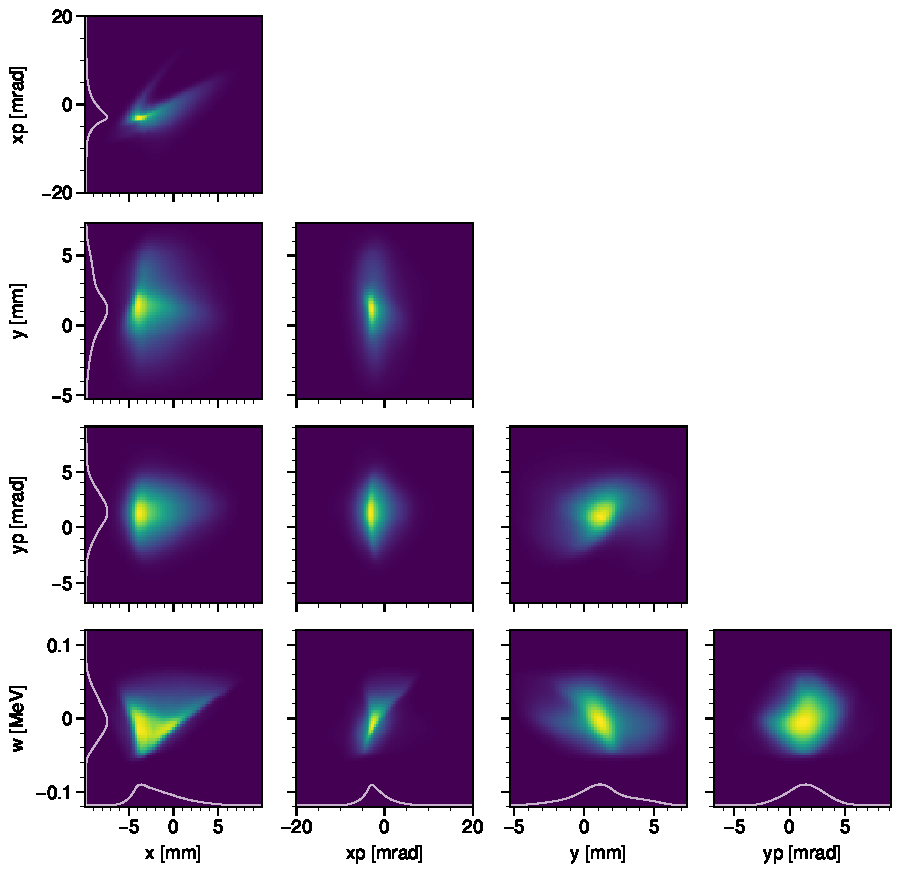
\includegraphics[width=\textwidth]{VS34_corner.pdf}
        \caption{}
        \label{fig:VS34_a}
    \end{subfigure}
    \hfill
    \hspace{0.1cm}
    \hfill
    \begin{subfigure}{0.48\textwidth}
        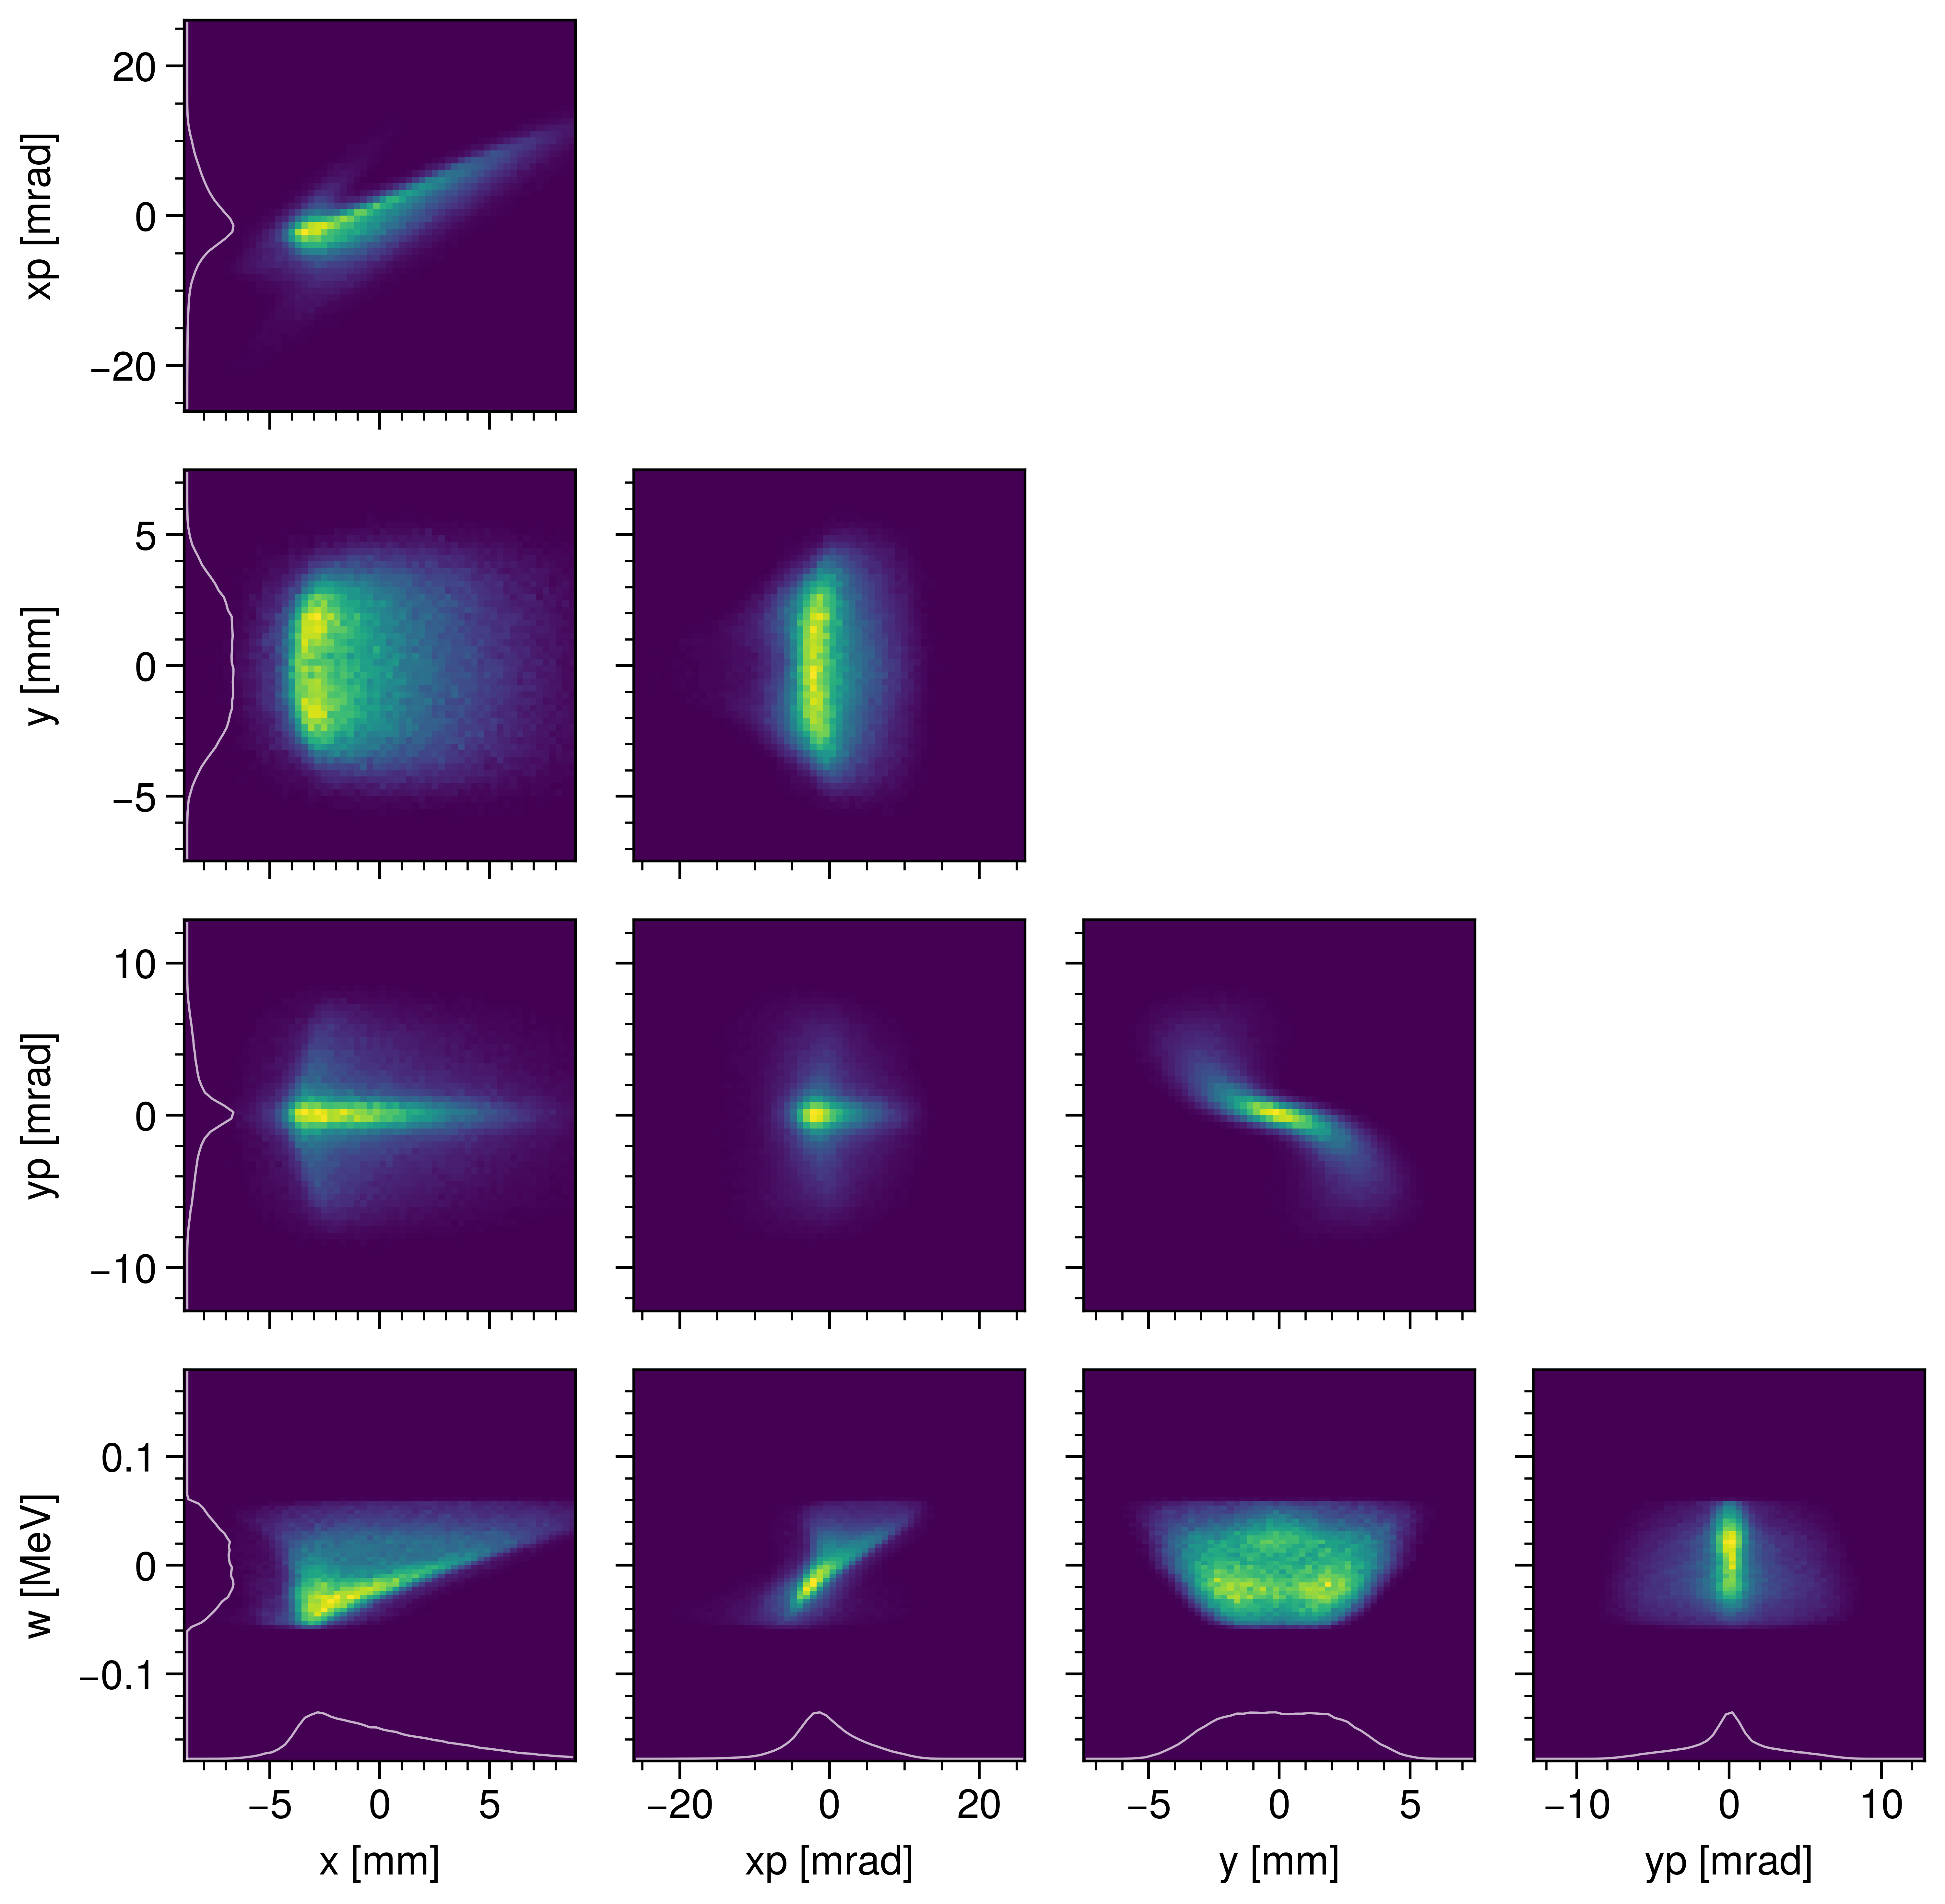
\includegraphics[width=\textwidth]{VS34_corner_sim.png}
        \caption{}
        \label{fig:VS34_b}
    \end{subfigure}
    \vfill
    % \vspace*{0.2cm}
    \vfill
    \begin{subfigure}{\textwidth}
        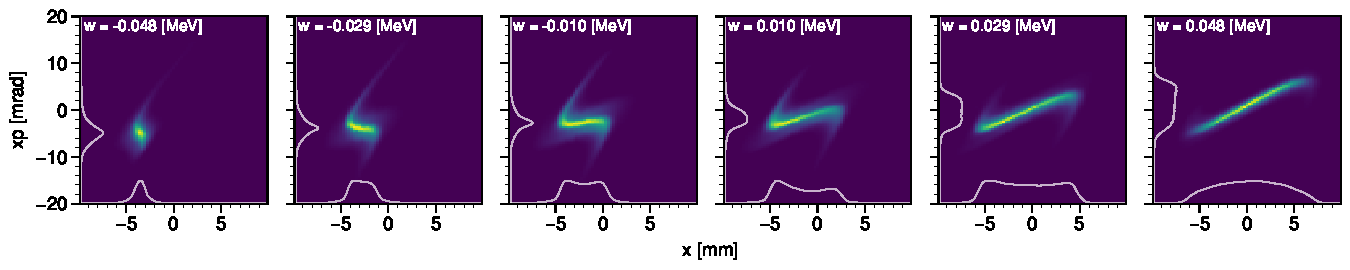
\includegraphics[width=\textwidth]{VS34_energy_slice.pdf}
        \caption{}
        \label{fig:VS34_c}
    \end{subfigure}
    \vfill
    % \vspace*{0.2cm}
    \vfill
    \begin{subfigure}{\textwidth}
        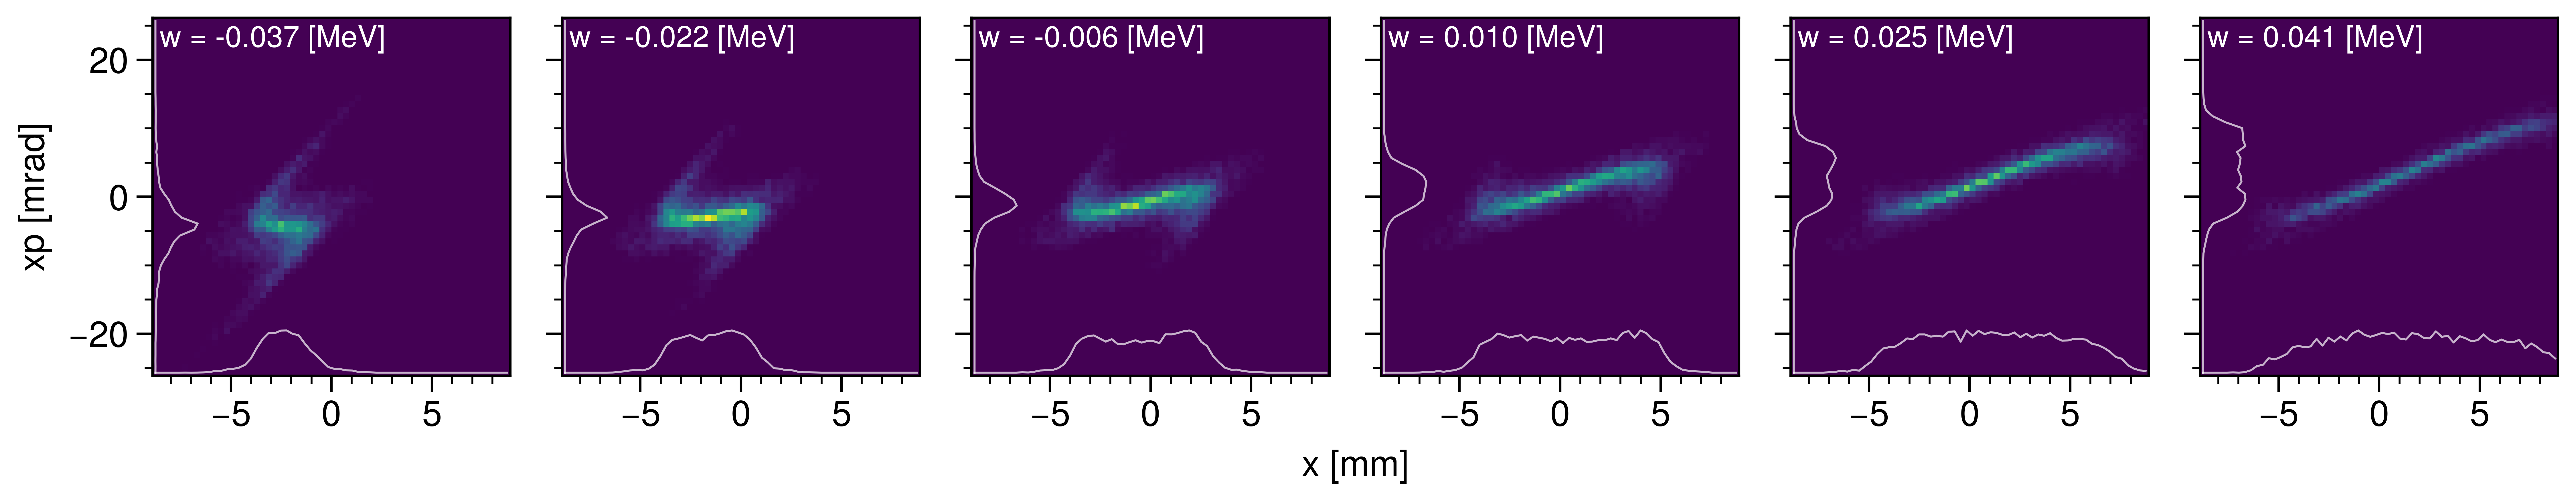
\includegraphics[width=\textwidth]{VS34_energy_slice_sim.png}
        \caption{}
        \label{fig:VS34_d}
    \end{subfigure}
    \caption{Comparison between the measured and simulated 5D phase space distribution at the second emittance station. (a) Measured 1D/2D projections. (b) Simulated 1D/2D projections. (c) Measured $x$-$x'$ distribution for different energy slices. (d) Simulated $x$-$x'$ distribution for different energy slices. The initial bunch in the simulation was generated by independently sampling measured 2D phase space distributions at the first emittance station.}
    \label{fig:VS34}
\end{figure*}
%

Slicing the array in this way selects only a small faction of the beam particles — vanishingly small when three or four dimensions are sliced. Therefore, the previous measurements do not characterize the extent of the hollow energy core in the full transverse phase space. This information is encoded in the 5D measurement: Fig.~\ref{fig:hollow_b} plots the energy distribution within a shrinking volume of transverse phase space. For each threshold $t$, we integrate the 5D array along the $w$ axis and locate all elements whose value is less than $t$ times the maximum element in the 4D array. We then mask these indices in the 5D array before projecting the array onto the $w$ axis. A hollow energy distribution begins to emerge at the $10^{-1}$ contour.

\subsection{Reconstructing the 6D distribution from 5D and 4D projections}

The effect of hidden high-dimensional features on halo formation and long-term beam dynamics is not yet known due to the lack of a realistic 6D simulation bunch.\footnote{
   Bunches produced by LEBT/RFQ simulations have qualitatively similar features to those seen in high-dimensional measurements, albeit large errors in the root-mean-square emittances. The simulated transport of these bunches through the SNS linac indicates that the correlations affect the root-mean-square beam sizes over time \cite{Ruisard2021-IPAC}.
} The present resolution and dynamic range of direct 6D measurements are too low to capture these features. It is therefore prudent to determine whether the 6D distribution can be recovered from the high-resolution, relatively high-dynamic-range 5D measurements described herein. The problem can be formulated as follows, letting $z$ and $z'$ be the longitudinal phase space coordinates: construct $f(x, x', y, y', z, z')$ consistent with the measured $f(x, x', y, y', z')$ and $f(x, x', z, z')$, where the latter is measured using two vertical slits and a BSM \cite{Ruisard2021-long}. 

We suggest several approaches here. A naive solution would be to set $f(x, x', y, y', z, z') = f(x, x', y, y', z') f(z)$; however, this assumes no correlation between $z$ and $z'$, which are strongly correlated in reality. A simple but promising approach is to generate a 5D particle distribution, then add the $z$-$z'$ correlation ``by hand", assuming $z \approx az' + \Delta$ where $a$ is a constant and $\Delta$ is a small random variable. This will be our first attempt.

More interesting is the case of an arbitrary $z$ distribution. An almost identical problem has been encountered in astrophysics: the Gaia satellite has measured the phase space coordinates of many stars in the Milky Way galaxy, but a large fraction of the measurements contain only five of the six coordinates. Bayesian neural networks have been employed to infer the missing coordinate \cite{}. 

Another approach is to treat the problem as a tomographic image reconstruction. For example, the Maximum Entropy (MENT) algorithm could be used, which selects the maximum entropy image among those consistent with the measured projections \cite{}. It is unknown if MENT (or other image reconstruction algorithms) can easily scale from two to six dimensions.


\section{5D simulation benchmark}

While the 6D measurement can only be performed at the first emittance station, the 5D measurement can be performed at either emittance station. This provides a unique opportunity for a 5D simulation benchmark. Fig.~\ref{fig:VS34} compares the measured 5D phase space distribution at the second emittance station to a simulation. The scan traversed a $64 \times 64 \times 64$ grid, collecting ? images pver ? hours. The simulation was performed with a 3D fast Fourier transform space charge solver on a ?x?x? mesh with one million macro-particles. THe initial simulation bunch was generated by independently sampling 2D measurements such that $f(x,x',y,y',z,z') = f(x,x')f(y,y')f(z,z')$. The reasonable agreement in $x$-$x'$-$w$ space — especially clear in the slice-emittances in Fig.~\ref{fig:VS34_c} and Fig.~\ref{fig:VS34_d} — was expected from previous successful benchmarks of the $x$-$x'$ distribution in \cite{Ruisard2021-IPAC}. The disagreement in the vertical plane is unresolved; it may be due to unidentified quadrupole misalignment or an offset of the beam centroid.



\section{Conclusion}

The Spallation Neutron Source (SNS) Beam Test Facility (BTF) has the ability to measure the full 6D phase space distribution of an intense ion beam. Such a measurement could lead to the accurate prediction of beam halo formation; however, the resolution and dynamic range of 6D measurements are currently two low to generate a realistic simulation bunch. 5D phase space measurements offer significant improvements in dynamic range and resolution. The 5D phase space distribution was measured at the first emittance station in the BTF. Hidden high-dimensional features in the beam core — previously measured only in small slices of the transverse phase space — were revisited. Several strategies to reconstruct the 6D distribution from the 5D measurement were suggested. Finally, the measured 5D phase space distribution at the end of the BTF beamline was used to benchmark a computer simulation. Reasonable agreement was found in the 3D $x$-$x'$-$w$ space. Significant disagreement remain in $y$-$y'$ space.

\section{ACKNOWLEDGEMENTS}
This material is based upon work supported by the U.S. Department of Energy, Office of Science, Office of High Energy Physics.
This manuscript has been authored by UT- Battelle, LLC under Contract No. DE-AC05-00OR22725 with the U.S. Department of Energy. This research used resources at the Spallation Neutron Source, a DOE Office of Science User Facility operated by the Oak Ridge National Laboratory.


% \section{Appendix}\label{app:A}

% \begin{figure}[!b]
%     \centering
%     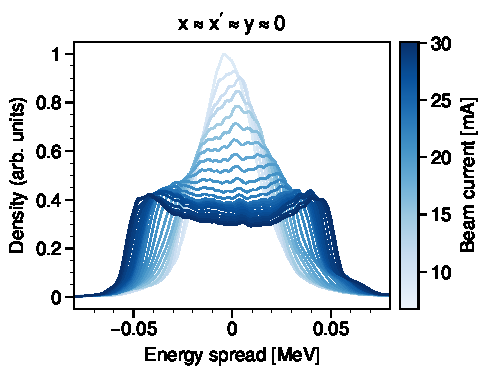
\includegraphics[width=0.8\columnwidth]{hollow_current.pdf}
%     \caption{Energy distribution of partial projections ($x \approx x' \approx y \approx 0$) of the beam as a function of the beam current. This reproduces Fig.~? from \cite{CatheyPRL} with a finer intensity scale.}
%     \label{fig:hollow_current}
% \end{figure}


\printbibliography

\end{document}
